\subsection{Topferkennung} \label{sec:Topferkennung}

\textit{(pro)} Als Sensor für die Topferkennung wurde der IR Distanzsensor von Sharp mit der Typenbezeichnung GP2Y0A41SK0F evaluiert. Er verfügt über einen Messbereich von 40mm... 300mm und ermittelt die Distanz durch Triangulation. Das Messsignal wird als Analog Pegel von 0V... 3.1V dargestellt.\\
Die Softwareauswertung der Topferkennung wurde aus Zeitgründen nicht mehr implementiert. Allerdings wurde ein Prove of Concept der Messmethode durchgeführt. Dabei wurde der genannten IR-Sensor mit einem ADC Port des FRDM-Boards verbunden. Es wurde eine Testmessung durchgeführt in der ein Blumentopf mit 14cm Durchmesser vor dem IR-Sensor, mit zwei verschiedenen Geschwindigkeiten, vorbeigeführt wurde. 

\begin{figure}[H]
	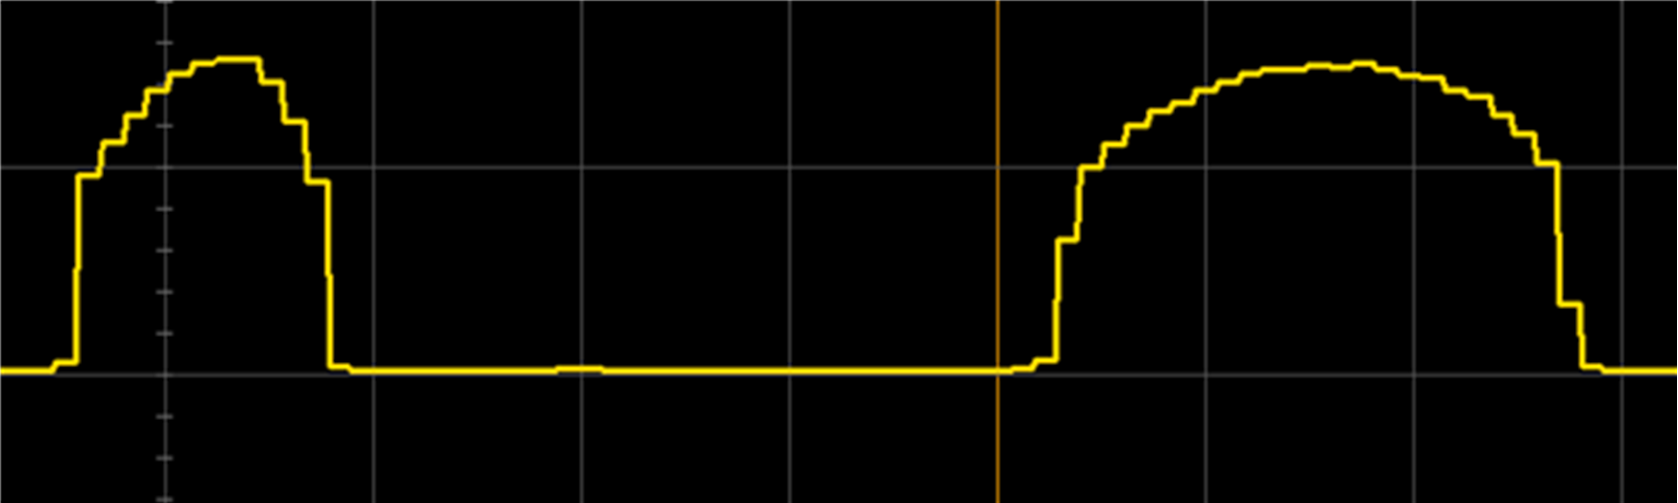
\includegraphics[width=1\textwidth]{Illustrationen/6-Umsetzung/IR_Sensor_Messung.png}
	\caption{Topferkennung, Testmessung}
	\label{fig:IR_Sensor_POC}
\end{figure}

Die Messung wurde mit der Software Segger J-Scope durchgeführt und ist in Abb. \ref{fig:IR_Sensor_POC} illustriert. Die Testmessung ist rein qualitativ und diente als Entscheidungsgrundlage für die Messmethode. Die Messdaten welche der Sensor liefert sind nicht linear und zusätzlich invertiert (hoher Pegel = kurze Messdistanz). Um absolute Werte für die Messdistanz zu bekommen, muss das Messsignal gemäss den Angaben im Datenblatt umgerechnet und über eine Lookup-Tabelle aufgelöst werden.

\subsubsection{Topfposition}
Die Informationen der Testmessung wurden als ausreichend empfunden um damit die Bewegungsphase eines Topfes zu erkennen und dementsprechend den Setzprozess auszulösen. Dafür wird der Sensor so platziert, dass sich der Topf im Stillstand direkt vor dem Sensor befindet. Durch die Stopp and Go Bewegung des Topkranzes der Topfmaschine TC5 entsteht ein Signalbild wie in Abb. \ref{fig:Signalbild_Topferkennung} illustriert.\\

\begin{figure}[H]
	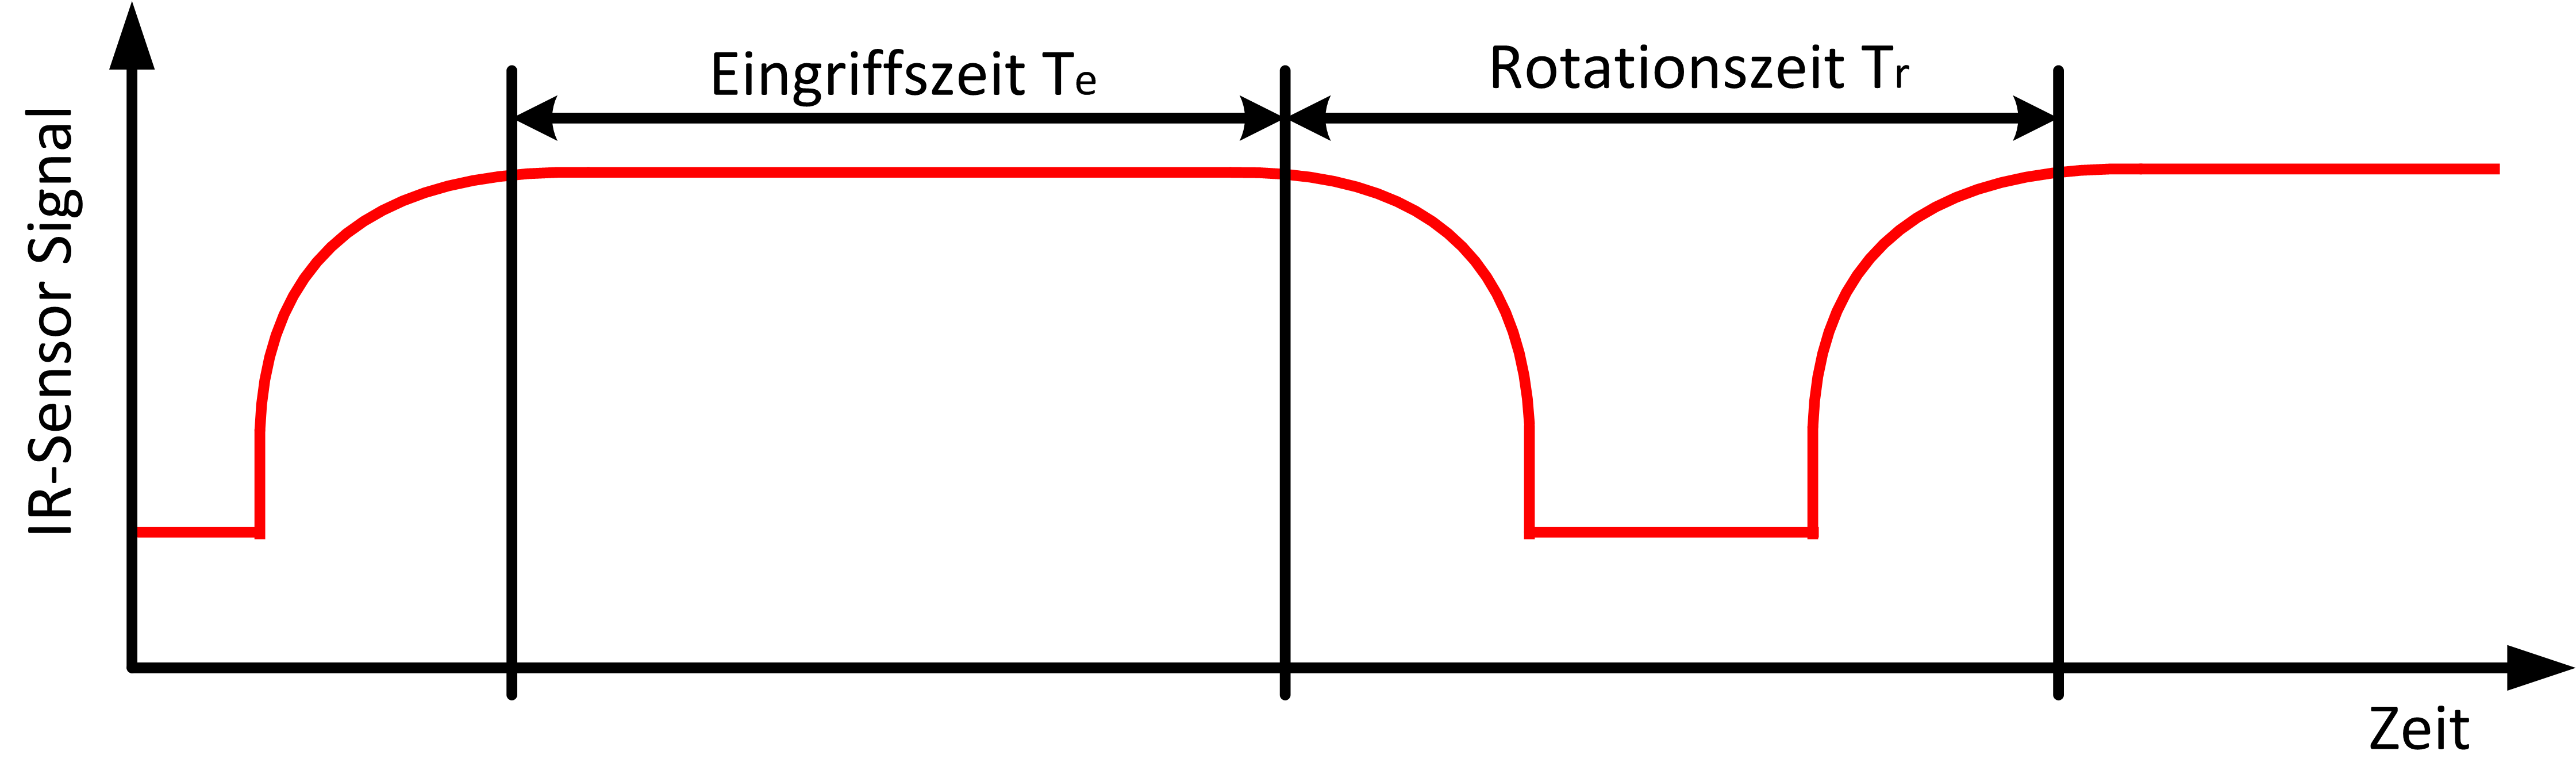
\includegraphics[width=0.9\textwidth]{Illustrationen/6-Umsetzung/Topferkennung_Messsignal.png}
	\caption{Topferkennung, Signalverlauf Topferkennung}
	\label{fig:Signalbild_Topferkennung}
\end{figure}

Um nun die Eingriffszeit T$_{e}$ bestimmen zu können, werden die Messwerte miteinander verglichen. Wenn die Messwerte in einem bestimmten Pegelbereich konstant bleiben kann davon ausgegangen werden, dass der Topf still steht.

\subsubsection{Topfgrösse}
Für die Messung der Topfgrösse reicht ein Sensor allerdings nur bedingt aus, da er aufgrund von überstehender Pflanzenerde eine Fehlmessung verursachen könnte. Um mit einer Distanzmessung zum Topf eine präzise Aussage über die Grösse des Topfes zu treffen, müsste zusätzlich die Geschwindigkeit des Topfkranzes erfasst werden. Eine weitere Möglichkeit wäre die Topfgrössenerkennung  durch Einsatz eines Echtzeit Bildverarbeitungssystems. Diese Sachverhalte führen zur Erkenntnis, dass die Topfgrössenerkennung einen zu grossen zeitlichen Aufwand für dieses Projekt bedeuten würde. Deshalb wird die Wunschanforderung nach einer automatischen Topfgrössenerkennung im Umfang dieses Projekts nicht realisiert.
